\section{Gain and loss of roles}

\textbf{Created by:} Arkopaul Sarkar \\
\textbf{Modified by:} Arkopaul Sarkar \\

\subsection*{Scenario Objective}

BFO roles are realizable entities external to the bearer and assigned within specific physical, social, or institutional contexts. A bearer can hold multiple roles over time or simultaneously, without ceasing to exist when roles change. However, BFO lacks constructs to indicate when roles begin or end. This scenario discussed the patterns around two subclasses of bfo:process, introduced by IOF Core to represent the the start and end of role. 

\subsection*{General Pattern Description}


\begin{figure}[ht]
    \centering
    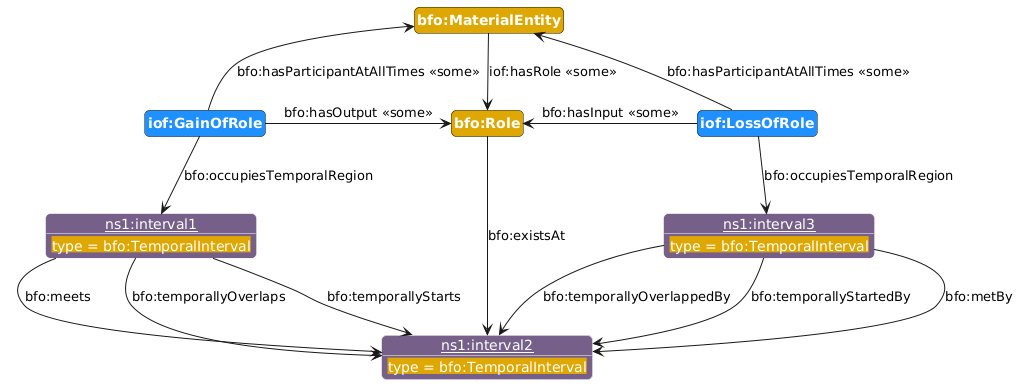
\includegraphics[scale=0.35]{scenarios/role-gain-loss/images/general-pattern.png}
    \label{fig:role-gain-loss-gp}
\end{figure}

Being specifically dependent continuants, BFO roles inheres in some independent containuant except spatial regions. The generic pattern diagram shows only material entity which bears the role (IOF provides a specialized property `has role' to only assign role to an entity) but some immaterial entities, such as sites and boundaries may also have a role. 

An intuitive way time bound the role is to use BFO `exists at' relation which links a temporal region to any entity. However, there is no constraints in BFO or IOF to obligate the role to be assigned to only one bearer during its existence, however, that may be the best practice. Moreover, the assignment and removal of a role from an entity may not have a sharp time point, e.g., an operator may need to go through a period of training to actually receive the role, or a product may need to go through testing and validation after it is bought and before it is registered as an asset (asset role) of the organization. Gain and loss of role classes provide user a way to assert actual start and end of a material entity carries a role. 

It can be noted that both `gain of role' and `loss of role' are BFO process, which signifies the processes of a material entity gaining and losing a role. The material entity bearing the role participates in these processes and the role it bears is the output of the gain-of-role process, and input of the loss-of-role process. Msot importantly, the interval for which the gain-of-role process occurs may meet, overlap, or start the interval for which the material entity bears the role and, conversely, the interval for which the loss-of-role process occurs may be met by, overlapped by, or started by the interval for which the material entity bears the role. This implies that the material entity may start bearing the role as soon as the process of gaining the role starts, or starts right after the role is gained, or somewhat in between. Similary, the material entity may stop bearining the role at the start of the losing the role process, or at the end of it, or somewhat in between. The user may select any combination of the above temporal relations depending on their requirements to assert the duration of the role. Some of these choices are explained in the use cases. 


\subsection*{Use Case: Assignment and Removal of a Safety Officer}

John K. Lee was appointed as the Safety Officer by the HR department of a manufacturing business on May 1, 2024. Following this decision, his role was formally registered in the company’s HR system on May 3, 2024. He officially began his duties at Plant A on May 6, 2024, taking on responsibilities related to workplace safety and compliance.

After serving in the role for nearly ten months, the HR department initiated the termination process of his appointment on March 31, 2025, upon completion of the planned term. Due to routine administrative handling, the role was formally deactivated in the system on April 4, 2025, which also marked John’s last working day as Safety Officer. He returned to his prior position thereafter.

\subsubsection*{Use-Case Pattern Description}

\begin{figure}[ht]
    \centering
    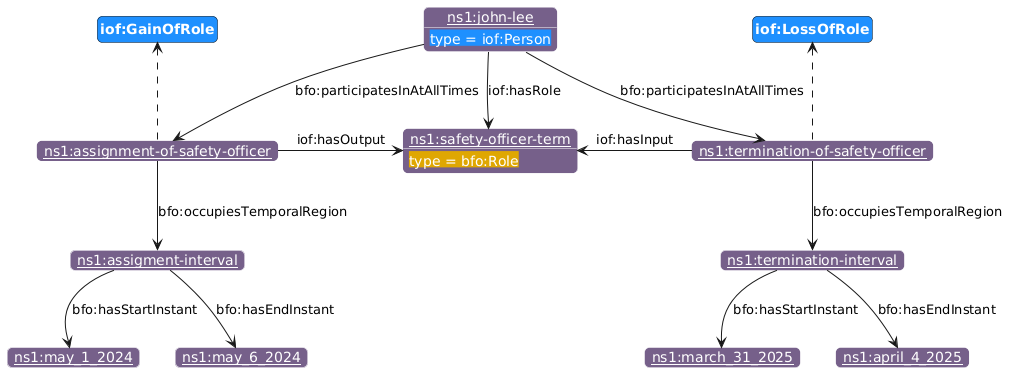
\includegraphics[scale=0.35]{scenarios/role-gain-loss/images/use-case1.png}
    \label{fig:role-gain-loss-gp}
\end{figure}

\subsubsection*{Data Mapping}

\begin{verbatim}
PREFIX xsd: <http://www.w3.org/2001/XMLSchema#>
PREFIX rdf: <http://www.w3.org/1999/02/22-rdf-syntax-ns#>
PREFIX ns1: <http://example.org/ns1#>
PREFIX bfo: <http://purl.obolibrary.org/obo/> 
PREFIX iof: <https://spec.industrialontologies.org/ontology/core/Core/>

INSERT DATA {
    
    ns1:john-lee a iof:Person;
    	bfo:BFO_0000166 ns1:assignment-of-safety-officer;
    	bfo:BFO_0000166 ns1:termination-of-safety-officer;
    	iof:hasRole ns1:safety-officer.
    
    ns1:safety-officer a bfo:BFO_0000023.

    ns1:assignment-of-safety-officer a iof:GainOfRole;
        bfo:occupiesTemporalRegion ns1:assignment-interval;
    	iof:hasOutput ns1:safety-officer.

    ns1:assignment-interval a bfo:BFO_0000202;
        bfo:BFO_0000222 ns1:assignment-start-time;
        bfo:BFO_0000224 ns1:assignment-end-time.
    
    ns1:assignment-start-time a bfo:BFO_0000203;
        iof:hasValueExpressionAtAllTimes ns1:assignment-start-time-value.

    ns1:assignment-end-time a bfo:TemporalInstant;
        iof:hasValueExpressionAtAllTimes ns1:assignment-end-time-value. 

    ns1:assignment-start-time-value iof:hasDateTimeInstantValue "2024-05-01T00:00:00Z"^^xsd:dateTime.
    ns1:assignment-end-time-value iof:hasDateTimeInstantValue "2024-05-06T00:00:00Z"^^xsd:dateTime.

    ns1:termination-of-safety-officer a iof:LossOfRole;  
        bfo:occupiesTemporalRegion ns1:termination-interval;
    	iof:hasInput ns1:safety-officer.

    ns1:termination-interval a bfo:BFO_0000202;
        bfo:BFO_0000222 ns1:termination-start-time;
        bfo:BFO_0000224 ns1:termination-end-time.
    
    ns1:termination-start-time a bfo:BFO_0000203;
        iof:hasValueExpressionAtAllTimes ns1:termination-start-time-value.

    ns1:termination-end-time a bfo:TemporalInstant;
        iof:hasValueExpressionAtAllTimes ns1:termination-end-time-value. 

    ns1:termination-start-time-value iof:hasDateTimeInstantValue "2025-03-31T00:00:00Z"^^xsd:dateTime.
    ns1:termination-end-time-value iof:hasDateTimeInstantValue "2025-04-04T00:00:00Z"^^xsd:dateTime.
}

\end{verbatim}

\subsubsection*{Data Validation}

\begin{verbatim}
PREFIX xsd: <http://www.w3.org/2001/XMLSchema#>
PREFIX rdf: <http://www.w3.org/1999/02/22-rdf-syntax-ns#>
PREFIX sh:  <http://www.w3.org/ns/shacl#>
PREFIX ns1: <http://example.org/ns1#>
PREFIX bfo: <http://purl.obolibrary.org/obo/> 
PREFIX iof: <https://spec.industrialontologies.org/ontology/core/Core/>
PREFIX ex:  <http://example.org/shapes#>

ex:AssignmentEventShape a sh:NodeShape ;
  sh:targetNode ns1:assignment-of-safety-officer ;
  sh:property [
    sh:path rdf:type ; sh:hasValue iof:GainOfRole
  ] ;
  sh:property [
    sh:path bfo:occupiesTemporalRegion ; sh:hasValue ns1:assignment-interval
  ] .

ex:AssignmentIntervalShape a sh:NodeShape ;
  sh:targetNode ns1:assignment-interval ;
  sh:property [
    sh:path rdf:type ; sh:hasValue bfo:BFO_0000202
  ] ;
  sh:property [
    sh:path bfo:BFO_0000222 ; sh:hasValue ns1:assignment-start-time
  ] ;
  sh:property [
    sh:path bfo:BFO_0000224 ; sh:hasValue ns1:assignment-end-time
  ] .

ex:AssignmentStartTimeShape a sh:NodeShape ;
  sh:targetNode ns1:assignment-start-time ;
  sh:property [
    sh:path rdf:type ; sh:hasValue bfo:BFO_0000203
  ] ;
  sh:property [
    sh:path iof:hasValueExpressionAtAllTimes ;
    sh:hasValue ns1:assignment-start-time-value
  ] .

ex:AssignmentEndTimeShape a sh:NodeShape ;
  sh:targetNode ns1:assignment-end-time ;
  sh:property [
    sh:path rdf:type ; sh:hasValue bfo:TemporalInstant
  ] ;
  sh:property [
    sh:path iof:hasValueExpressionAtAllTimes ;
    sh:hasValue ns1:assignment-end-time-value
  ] .

ex:AssignmentStartValueShape a sh:NodeShape ;
  sh:targetNode ns1:assignment-start-time-value ;
  sh:property [
    sh:path iof:hasDateTimeInstantValue ;
    sh:hasValue "2024-05-01T00:00:00Z"^^xsd:dateTime
  ] .

ex:AssignmentEndValueShape a sh:NodeShape ;
  sh:targetNode ns1:assignment-end-time-value ;
  sh:property [
    sh:path iof:hasDateTimeInstantValue ;
    sh:hasValue "2024-05-06T00:00:00Z"^^xsd:dateTime
  ] .
\end{verbatim}

\subsection*{Use Case: Shift Monitoring}

A 24-hour control room is staffed continuously by three operators working in rotating shifts of approximately eight hours each. A short change-over period of about ten minutes ensures seamless transition between shifts, during which both incoming and outgoing operators are present. Each operator’s shift officially begins upon arrival in the control room and ends upon departure, with all such events recorded in a logbook.

On 28th May 2016, the logbook captured a sequence of arrivals, departures, and two incidents. The organization seeks to use this information to answer two key monitoring questions in a structured way to audit staff transitions, maintain accountability, and ensure operational continuity during critical events. 
\begin{enumerate}
    \item which operator formally took over duties from whom during each shift handover?
    \item which operators were physically present in the control room at the precise times when incidents occurred?
\end{enumerate}

Logbook entries on 28th May 2016.

\begin{verbatim}
[2016-05-28T00:03:00Z] Operator 1 arrived for change-over. 
[2016-05-28T00:10:00Z] Operator 3 left the control.
[2016-05-28T03:24:00Z] Incident 1 is observed.
[2016-05-28T03:26:00Z] Incident 1 is stopped.
[2016-05-28T07:58:00Z] Operator 2 arrived for change-over.
[2016-05-28T08:07:00Z] Operator 1 left the control.
[2016-05-28T16:01:00Z] Operator 3 arrived for change-over.
[2016-05-28T16:05:00Z] Incident 2 is observed.
[2016-05-28T16:08:00Z] Operator 2 left the control.
[2016-05-28T23:43:00Z] Incident 3 is observed.
\end{verbatim}

\subsubsection*{Use-Case Pattern Description}

